% Autor: Mauricio S. Matias Conde

% Clase de Documento, formato libro
\documentclass[12pt,letterpaper]{book}
% Paquete para el soporte de idiomas
\usepackage[spanish,es-tabla]{babel}
% Paquete para la manipulación de imágenes.
\usepackage{graphicx}
% Paquete para la referencias links y marcadores en el menu del pdf
\usepackage{hyperref}
% Márgenes de la hoja
\usepackage[top=2cm,bottom=2cm,left=3cm,right=2cm]{geometry}
% Paquete para encabezados o pies de página.
\usepackage{fancyhdr}   
% Paquete para la prevensión de aparición 
% de pies de página, encabezados y numeración.
\usepackage{emptypage}  
% Paquete para la adecuación de cuadros y tablas.
\usepackage{float}      
% Paquete que permite la construcción de tablas
% que abarquen mas de una página.
\usepackage{longtable}       
% Paquete que ofrece el soporte de citación 
% estilo APA.
\usepackage{apacite} 
% Paquetes para el uso de fórmulas matemáticas.
\usepackage{amsmath, amsthm, amssymb}
% Paquete para la inclusión de Anexos
\usepackage{appendix}
% Paquete para la graficación
\usepackage{tikz}
\usetikzlibrary{shapes,arrows}
% Paquete para la incrustación de datos personales
\usepackage{configs/docstyle}

\begin{document}
    \renewcommand{\BOthers}[1]{et al.\hbox{}}
\renewcommand{\BAvailFrom}[1]{Recuperado de\hbox{}}
\renewcommand{\BRetrievedFrom}[1]{Recuperado de }
\renewcommand{\BRetrieved}[1]{}

\renewcommand{\appendixname}{Anexos}
\renewcommand{\appendixtocname}{Anexos}
\renewcommand{\appendixpagename}{Anexos}

% Configuración de las formas en la graficación de diagramas de flujo
\tikzstyle{decision} = [diamond, draw, fill=blue!15, 
  text width=4.5em, text badly centered, node distance=3cm, inner sep=0pt]
\tikzstyle{block} = [rectangle, draw, fill=blue!15, 
  text width=5em, text centered, rounded corners, minimum height=4em]
\tikzstyle{line} = [draw, -latex']
\tikzstyle{cloud} = [draw, ellipse,fill=red!15, node distance=3cm,
  minimum height=2em]
    \newgeometry{top=2cm,bottom=2cm,left=2cm,right=2cm}
\begin{titlepage}
    \begin{minipage}{2.7cm}
        \begin{center}
            
\includegraphics[width=3cm,height=3cm]{img/logo_universidad.png}
        \end{center}
    \end{minipage}
    \hfill
    \begin{minipage}{11cm}
        \begin{center}
            \large{ \textbf{\MakeUppercase{\nombreUniversidad}} }\\
            \normalsize{ \textbf{\MakeUppercase{\nombreFacultad}} }\\
            \small{ \textbf{\MakeUppercase{\nombreCarrera}} }
        \end{center}
    \end{minipage}
    \hfill
    \begin{minipage}{3.0cm}
        \begin{center}
            
\includegraphics[width=3.0cm,height=3.0cm]{img/logo_facultad.png}
        \end{center}
    \end{minipage}
    \vspace{5cm}\\
    \begin{center}
        \MakeUppercase{\nombreProyecto}
    \end{center}
    \vspace{4cm}
    \descripcion\\

    \vspace{2cm}
    \textnormal{\textbf{Presentado por:} \nombreAutor}\\

    \vspace{0.3cm}
    \textnormal{\textbf{Tutor:} \nombreTutor}\\

    \vspace{3.5cm}
    \begin{center}
        \textbf{\MakeUppercase{\nombreCiudadPais}}\\
        \fecha
    \end{center}
\end{titlepage}
\restoregeometry
    
    \frontmatter
    \chapter{Dedicatoria}
A mi abuelo que me enseñó a no parar de
estudiar y aprender, a mi abuela que me
transmitió su curiosidad, a mi hermano que
me extiende la mano cuando tengo problemas y a 
mi querida madre que me impregnó de su enorme
fuerza de voluntad y paciencia.
    \chapter{Agradecimientos}
Agradezco a mis amigos y amigas que siempre
hacen más entretenido el día, ayudandome a recordar
que los límites no existen, a pesar de que no siempre
los tenga en mente, los tengo en el corazón.\\

Agradezco también a la vida por todas aquellas personas 
que por azares del destino llegué a conocer, con las 
cuales he pasado inolvidables momentos, mañanas de estudio,
tardes de juegos y paseos, noches de cuestionamientos 
filosóficos y charlas sin sentido.\\
    \tableofcontents
    \listoffigures
    \listoftables
    
    \mainmatter     
    \chapter{Recursos LaTeX}

\begin{center}
    \textit{En que consiste este capítulo (Aquí).}
\end{center}

\section{Fuente}

\subsection{Familia}
{\ttfamily typewriter (máquina de escribir)}

{\sffamily sans serif}

{\rmfamily roman}

\subsection{Forma}
\textbf{texto en negritas}\\
\textit{texto en itálicas}\\
\textsl{texto inclinado}\\
\texttt{texto en estilo máquina de escribir}\\
\textsc{texto en mayúsculas pequeñas}

\subsection{Tamaño}
{\tiny texto de prueba}\\
{\scriptsize texto de prueba}\\
{\footnotesize texto de prueba}\\
{\small texto de prueba}\\
{\normalsize texto de prueba}\\
{\large texto de prueba}\\
{\Large texto de prueba}\\
{\LARGE texto de prueba}\\
{\huge texto de prueba}\\
{\Huge texto de prueba}

\section{Listado}

\subsection{No numerados}
\begin{itemize}
    \item Item 1
    \item Item 2
    \item Item 3
\end{itemize}

\subsection{Numerados}
\begin{enumerate}
    \item Item 1
    \item Item 2
    \item Item 3
\end{enumerate}


\section{Referenciación con APA}

\subsection{Citación como parte de párrafo}

\subsection*{Un autor}

Como menciona \citeA{libro:ejemplo}, no es la única
forma de citar.\\

\subsection*{Varios autores}

Como menciona \citeA{libro:ejemplo_varios_autores}, no es la única
forma de citar.\\

\subsection{Citación en la parte final}

\subsection*{Un autor}

Duis fringilla tristique neque. Sed interdum libero ut metus.
Pellentesque placerat. Nam rutrum augue a leo. Morbi sed 
elit sit amet ante lobortis sollicitudin.Praesent blandit 
blandit mauris citumoris totalis. \cite{libro:ejemplo}.

\subsection*{Varios autores}

Duis fringilla tristique neque. Sed interdum libero ut metus.
Pellentesque placerat. Nam rutrum augue a leo. Morbi sed 
elit sit amet ante lobortis sollicitudin.Praesent blandit 
blandit mauris citumoris totalis. \cite{libro:ejemplo_varios_autores}.

\subsection{Citación con número de página}

Como menciona \citeA[p.~5]{libro:ejemplo}, no es la única
forma de citar.\\

Duis fringilla tristique neque. Sed interdum libero ut metus.
Pellentesque placerat. Nam rutrum augue a leo. Morbi sed 
elit sit amet ante lobortis sollicitudin.Praesent blandit 
blandit mauris citumoris totalis. \cite[p.~7-12]{libro:ejemplo_varios_autores}.

\subsection{Citación Anexos}
Citación ()

\section{Figuras}
Referenciando a la figura \ref{fig:ejemplo}.

\begin{figure}[H]
    \begin{center}
        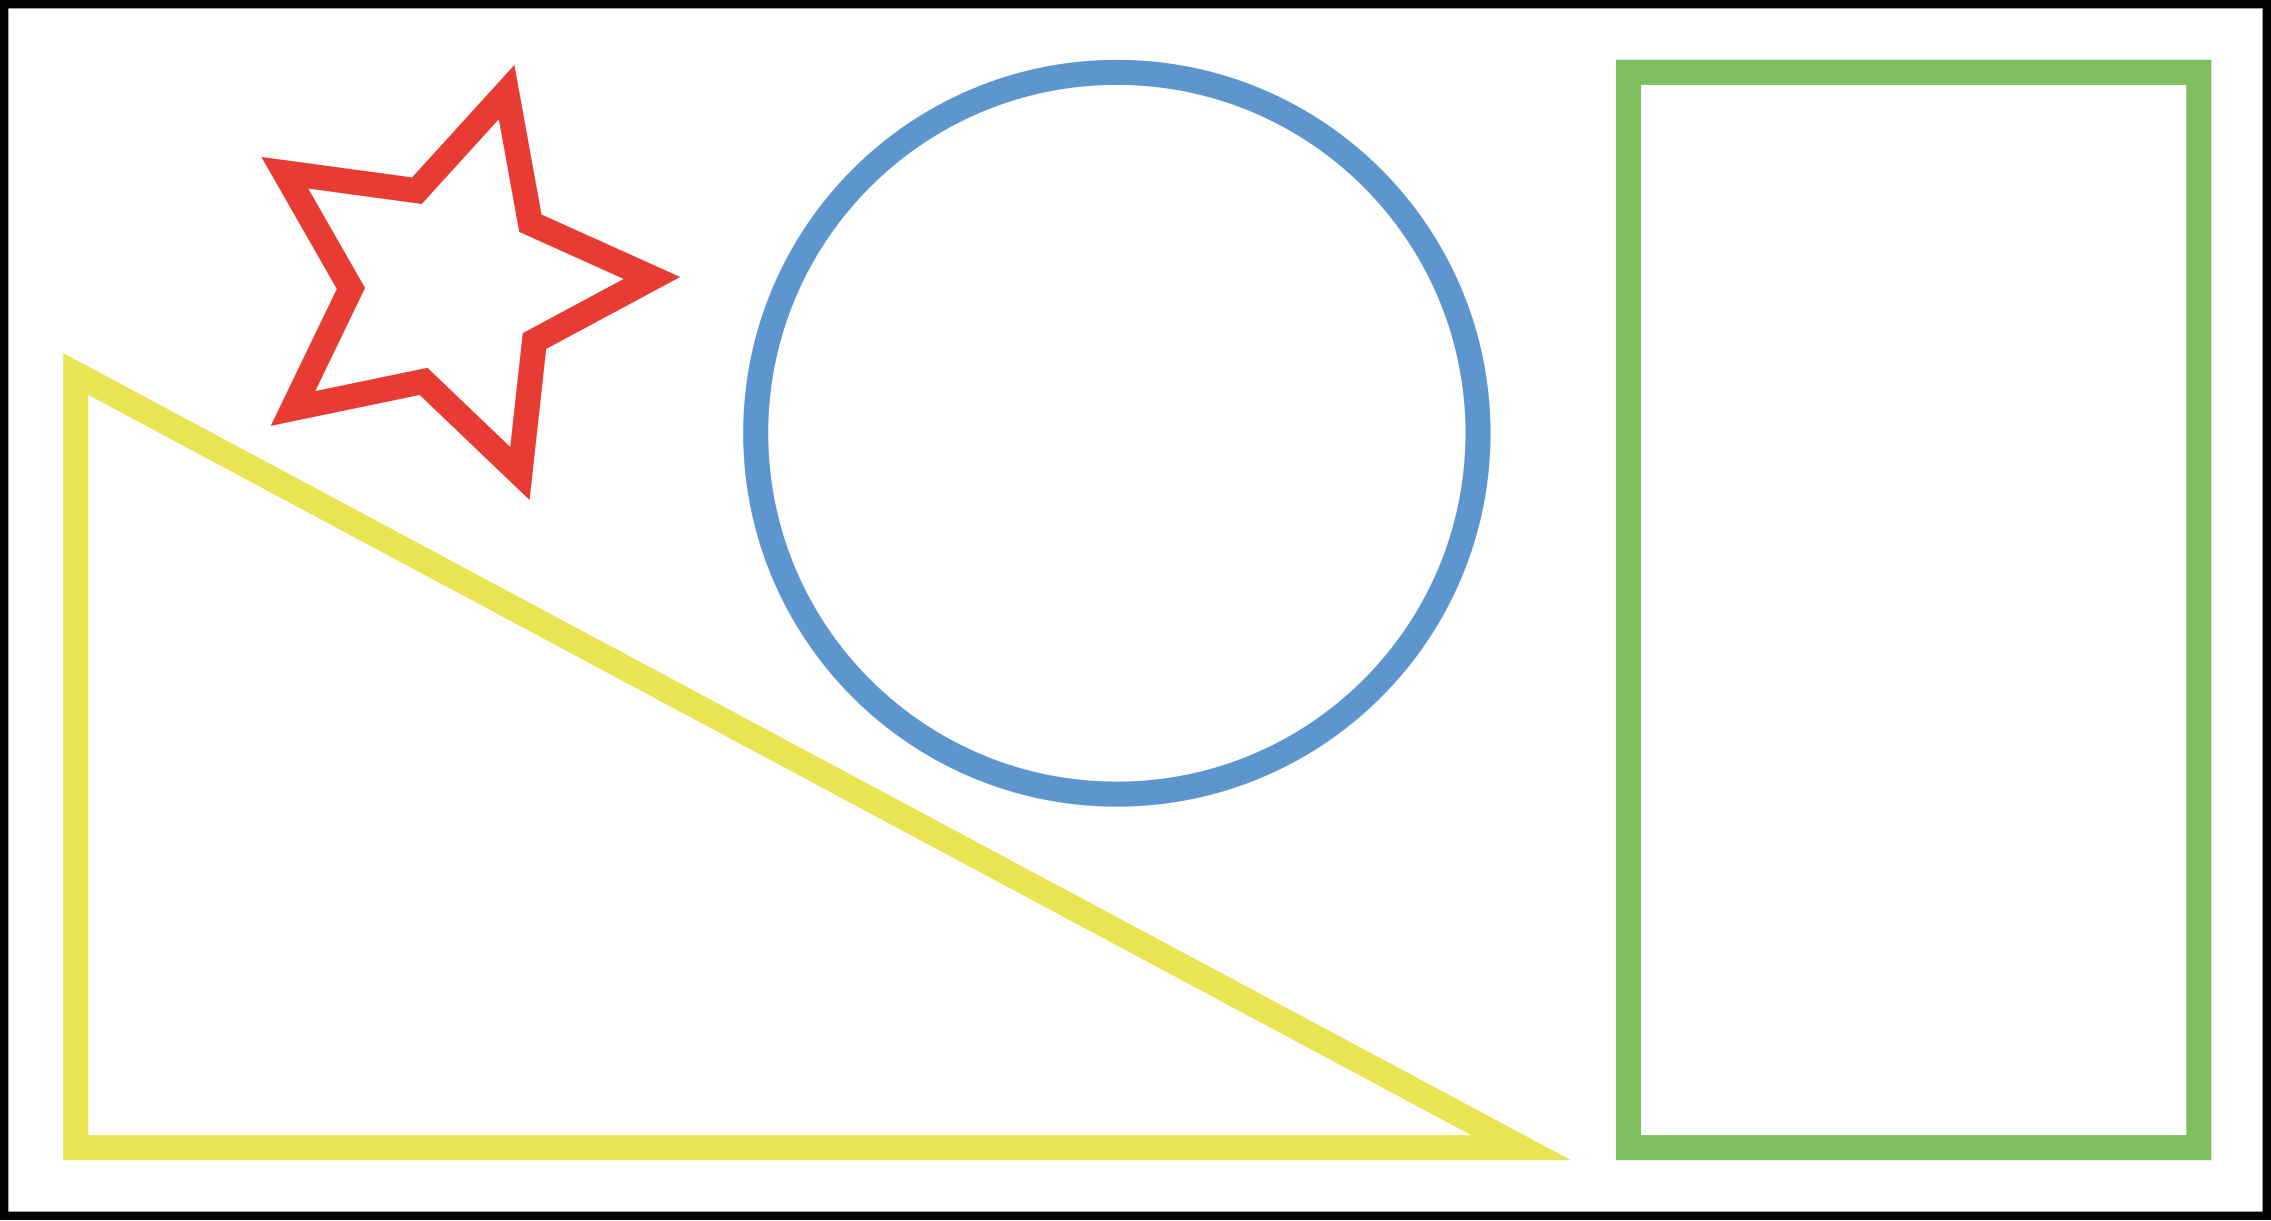
\includegraphics[width=8cm]{img/figura_ejemplo.png}
    \end{center}
    \caption{Explicación de la figura (Aquí)}
    Fuente: Adaptada de Apellido, N. (2000) \textit{Nombre del libro}.
    Editorial o universidad que lo publicó.
    \label{fig:ejemplo}
\end{figure}

\section{Tablas}

\subsection{Corto}
Referenciando a la tabla \ref{tabla:ejemplo}.\\

\begin{table}[H]
    \caption{Título de la tabla}
    \label{tabla:ejemplo}
    \begin{center}
        \begin{tabular}{c|c|c|c|}
            \cline{2-4}
            & \textbf{Columna 1} & \textbf{Columna 2} & \textbf{Columna 3} \\ \hline
            \multicolumn{1}{|c|}{\textbf{Fila 1}} & item               & item               & item               \\ \hline
            \multicolumn{1}{|c|}{\textbf{Fila 2}} & item               & item               & item               \\ \hline
            \multicolumn{1}{|c|}{\textbf{Fila 3}} & item               & item               & item               \\ \hline
        \end{tabular}
    \end{center}
    Nota. Extraída de Apellido, N. (2000) \textit{Nombre del libro}.
    Editorial o universidad que lo publicó.
\end{table}

\subsection{Multipágina}
Stique neque. Sed interdum libero ut metus.
Pellentesque placerat. Nam rutrum augue a leo. Morbi sed 
elit sit amet ante lobortis sollicitudin.Praesent blandit 
blandit mauris. Praesent lectus tellus, aliquet aliquam,
luctus a, egestas a, turpis.Mauris lacinia lorem sit amet
ipsum. Nunc quis urna dictum turpis accumsan semper. Tabla
\ref{tabla:tabla_largo_ejemplo}.\\

\begin{longtable}{p{2cm}|p{3cm}|p{3cm}|p{3cm}|p{3cm}|}
    \caption{Titulo de tabla multipágina} \label{tabla:tabla_largo_ejemplo} \\
    \cline{2-5}
    \multicolumn{1}{l|}{} & \multicolumn{1}{c|}{\textbf{Columna 1}} & \multicolumn{1}{c|}{\textbf{Columna 2}} & \multicolumn{1}{c|}{\textbf{Columna 3}} & \multicolumn{1}{c|}{\textbf{Columna 4}}\\ \hline
    \endfirsthead

    \multicolumn{5}{c}{{\tablename{} \thetable{} -- Continuación de tabla previa}} \\
    \multicolumn{5}{l}{} \\
    \cline{2-5}
    \multicolumn{1}{l|}{} & \multicolumn{1}{c|}{\textbf{Columna 1}} & \multicolumn{1}{c|}{\textbf{Columna 2}} & \multicolumn{1}{c|}{\textbf{Columna 3}} & \multicolumn{1}{c|}{\textbf{Columna 4}}\\ \hline
    \endhead

    \multicolumn{5}{c}{{Continua en la siguiente página.}} \\
    \endfoot

    \multicolumn{5}{l}{} \\
    \multicolumn{5}{l}{Nota. Extraída de Apellido, N. (2000) \textit{Nombre del libro}. Editorial o universidad que lo publicó.} \\
    \endlastfoot

    \multicolumn{1}{|c|}{\textbf{Fila 1}} & Lorem ipsum dolor sit amet, consectetuer adipiscing elit. & Lorem ipsum dolor sit amet, consectetuer adipiscing elit. & Lorem ipsum dolor sit amet, consectetuer adipiscing elit. & Lorem ipsum dolor sit amet, consectetuer adipiscing elit. \\ \hline
    \multicolumn{1}{|c|}{\textbf{Fila 2}} & Lorem ipsum dolor sit amet, consectetuer adipiscing elit. & Lorem ipsum dolor sit amet, consectetuer adipiscing elit. & Lorem ipsum dolor sit amet, consectetuer adipiscing elit. & Lorem ipsum dolor sit amet, consectetuer adipiscing elit. \\ \hline
    \multicolumn{1}{|c|}{\textbf{Fila 3}} & Lorem ipsum dolor sit amet, consectetuer adipiscing elit. & Lorem ipsum dolor sit amet, consectetuer adipiscing elit. & Lorem ipsum dolor sit amet, consectetuer adipiscing elit. & Lorem ipsum dolor sit amet, consectetuer adipiscing elit. \\ \hline
    \multicolumn{1}{|c|}{\textbf{Fila 4}} & Lorem ipsum dolor sit amet, consectetuer adipiscing elit. & Lorem ipsum dolor sit amet, consectetuer adipiscing elit. & Lorem ipsum dolor sit amet, consectetuer adipiscing elit. & Lorem ipsum dolor sit amet, consectetuer adipiscing elit. \\ \hline
    \multicolumn{1}{|c|}{\textbf{Fila 5}} & Lorem ipsum dolor sit amet, consectetuer adipiscing elit. & Lorem ipsum dolor sit amet, consectetuer adipiscing elit. & Lorem ipsum dolor sit amet, consectetuer adipiscing elit. & Lorem ipsum dolor sit amet, consectetuer adipiscing elit. \\ \hline
    \multicolumn{1}{|c|}{\textbf{Fila 6}} & Lorem ipsum dolor sit amet, consectetuer adipiscing elit. & Lorem ipsum dolor sit amet, consectetuer adipiscing elit. & Lorem ipsum dolor sit amet, consectetuer adipiscing elit. & Lorem ipsum dolor sit amet, consectetuer adipiscing elit. \\ \hline  
    \multicolumn{1}{|c|}{\textbf{Fila 7}} & Lorem ipsum dolor sit amet, consectetuer adipiscing elit. & Lorem ipsum dolor sit amet, consectetuer adipiscing elit. & Lorem ipsum dolor sit amet, consectetuer adipiscing elit. & Lorem ipsum dolor sit amet, consectetuer adipiscing elit. \\ \hline    
    \multicolumn{1}{|c|}{\textbf{Fila 8}} & Lorem ipsum dolor sit amet, consectetuer adipiscing elit. & Lorem ipsum dolor sit amet, consectetuer adipiscing elit. & Lorem ipsum dolor sit amet, consectetuer adipiscing elit. & Lorem ipsum dolor sit amet, consectetuer adipiscing elit. \\ \hline    
    \multicolumn{1}{|c|}{\textbf{Fila 9}} & Lorem ipsum dolor sit amet, consectetuer adipiscing elit. & Lorem ipsum dolor sit amet, consectetuer adipiscing elit. & Lorem ipsum dolor sit amet, consectetuer adipiscing elit. & Lorem ipsum dolor sit amet, consectetuer adipiscing elit. \\ \hline    
    \multicolumn{1}{|c|}{\textbf{Fila 10}} & Lorem ipsum dolor sit amet, consectetuer adipiscing elit. & Lorem ipsum dolor sit amet, consectetuer adipiscing elit. & Lorem ipsum dolor sit amet, consectetuer adipiscing elit. & Lorem ipsum dolor sit amet, consectetuer adipiscing elit. \\ \hline    
    \multicolumn{1}{|c|}{\textbf{Fila 11}} & Lorem ipsum dolor sit amet, consectetuer adipiscing elit. & Lorem ipsum dolor sit amet, consectetuer adipiscing elit. & Lorem ipsum dolor sit amet, consectetuer adipiscing elit. & Lorem ipsum dolor sit amet, consectetuer adipiscing elit. \\ \hline    
    \multicolumn{1}{|c|}{\textbf{Fila 12}} & Lorem ipsum dolor sit amet, consectetuer adipiscing elit. & Lorem ipsum dolor sit amet, consectetuer adipiscing elit. & Lorem ipsum dolor sit amet, consectetuer adipiscing elit. & Lorem ipsum dolor sit amet, consectetuer adipiscing elit. \\ \hline    
\end{longtable}

\section{Fórmulas matemáticas}

\section*{Simple}
\begin{equation}
    e^{i\pi} + 1 = 0
    \label{eq:euler}
\end{equation}

\section*{Matrices}
\begin{equation}
    \left[
    \begin{matrix}
     a & b & c \\
     d & e & f \\
     g & h & i
    \end{matrix}
    \right]
    \label{eq:matriz}
\end{equation}

\section*{Límites}
\begin{equation}
    \lim_{x\rightarrow\infty}\frac{3+x}{x^2} 
    \label{eq:limites}
\end{equation}
    
    \backmatter
    \bibliographystyle{apacite}
    \bibliography{bibliografia}

    \appendix
    \clearpage
    \addappheadtotoc
    \appendixpage
    \chapter{Anexo A: Título de Anexo A}

Contenido de Anexo A
    \chapter{Anexo B: Título de Anexo B}

Contenido de Anexo B
    
\end{document}